\documentclass{standalone}
\usepackage{tikz}
\usetikzlibrary{patterns, positioning}


\begin{document}
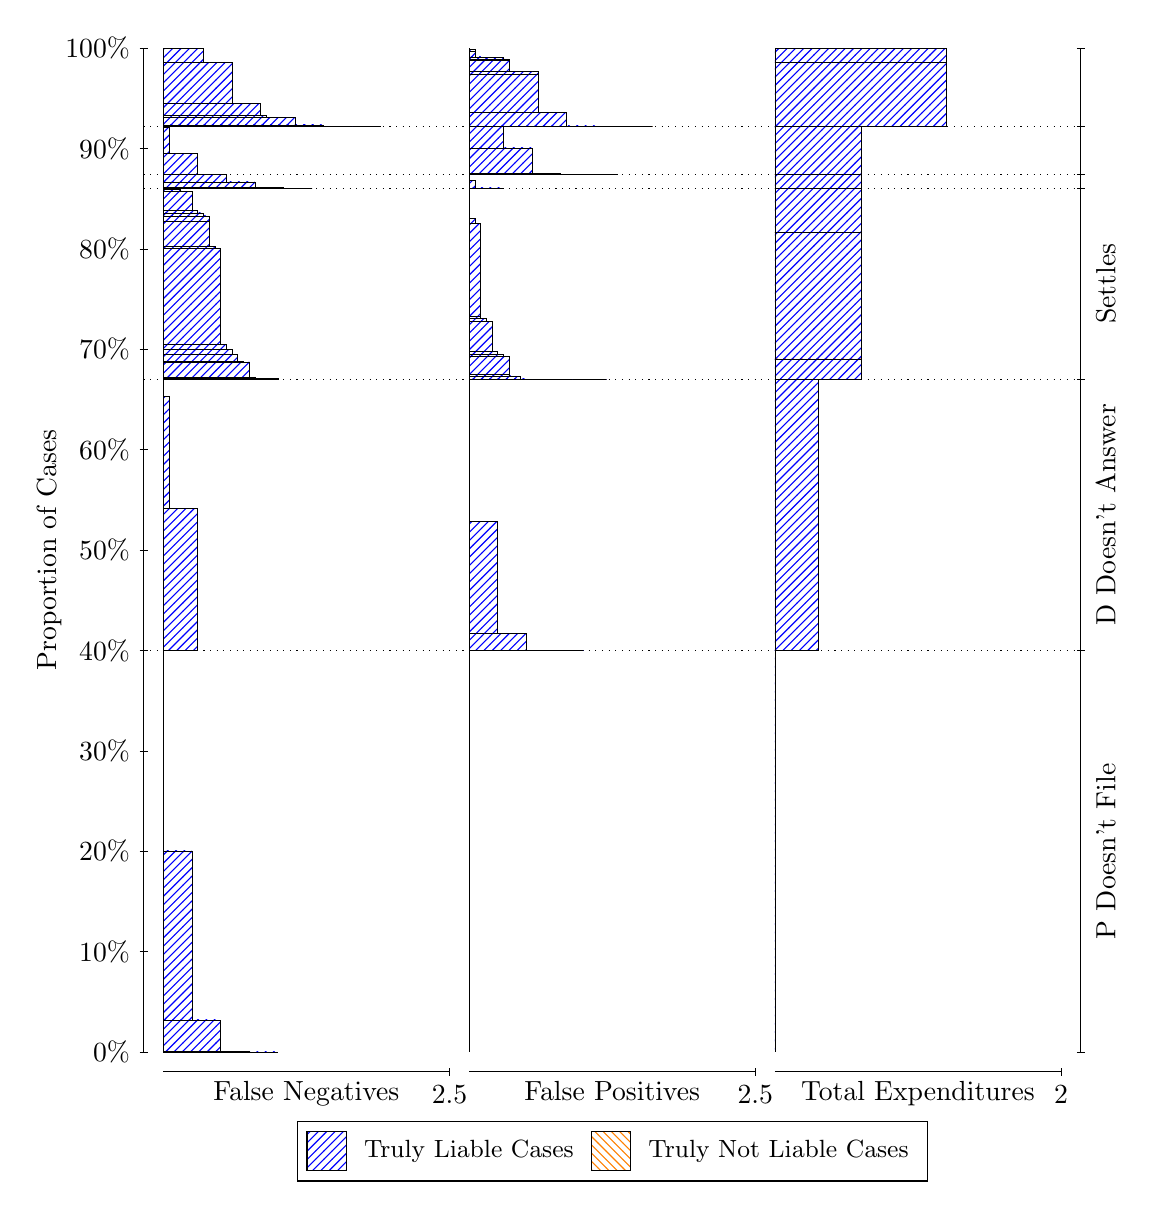
\begin{tikzpicture}
\draw[black, very thin] (1.5,1.75) -- (1.5,14.5);
\node[rotate=90, text=black, anchor=center] at (0.3, 8.125) {Proportion of Cases};
\draw[black, very thin] (1.45,1.75) -- (1.55,1.75);
\node[text=black, anchor=east] at (1.45, 1.75) {0\%};
\draw[black, very thin] (1.45,3.025) -- (1.55,3.025);
\node[text=black, anchor=east] at (1.45, 3.025) {10\%};
\draw[black, very thin] (1.45,4.3) -- (1.55,4.3);
\node[text=black, anchor=east] at (1.45, 4.3) {20\%};
\draw[black, very thin] (1.45,5.575) -- (1.55,5.575);
\node[text=black, anchor=east] at (1.45, 5.575) {30\%};
\draw[black, very thin] (1.45,6.85) -- (1.55,6.85);
\node[text=black, anchor=east] at (1.45, 6.85) {40\%};
\draw[black, very thin] (1.45,8.125) -- (1.55,8.125);
\node[text=black, anchor=east] at (1.45, 8.125) {50\%};
\draw[black, very thin] (1.45,9.4) -- (1.55,9.4);
\node[text=black, anchor=east] at (1.45, 9.4) {60\%};
\draw[black, very thin] (1.45,10.675) -- (1.55,10.675);
\node[text=black, anchor=east] at (1.45, 10.675) {70\%};
\draw[black, very thin] (1.45,11.95) -- (1.55,11.95);
\node[text=black, anchor=east] at (1.45, 11.95) {80\%};
\draw[black, very thin] (1.45,13.225) -- (1.55,13.225);
\node[text=black, anchor=east] at (1.45, 13.225) {90\%};
\draw[black, very thin] (1.45,14.5) -- (1.55,14.5);
\node[text=black, anchor=east] at (1.45, 14.5) {100\%};

\draw[black, very thin] (13.4,1.75) -- (13.4,14.5);
\draw[black, very thin] (13.35,1.75) -- (13.45,1.75);
\node[anchor=west] at (13.35, 1.75) {};
\draw[black, very thin] (13.35,6.8489) -- (13.45,6.8489);
\node[anchor=west] at (13.35, 6.8489) {};
\draw[black, very thin] (13.35,10.294) -- (13.45,10.294);
\node[anchor=west] at (13.35, 10.294) {};
\draw[black, very thin] (13.35,12.721) -- (13.45,12.721);
\node[anchor=west] at (13.35, 12.721) {};
\draw[black, very thin] (13.35,12.894) -- (13.45,12.894);
\node[anchor=west] at (13.35, 12.894) {};
\draw[black, very thin] (13.35,13.504) -- (13.45,13.504);
\node[anchor=west] at (13.35, 13.504) {};
\draw[black, very thin] (13.35,14.5) -- (13.45,14.5);
\node[anchor=west] at (13.35, 14.5) {};

\draw[black, very thin, pattern color=blue, pattern=north east lines] (1.75,1.75) rectangle (3.2033,1.75);
\draw[black, very thin, pattern color=blue, pattern=north east lines] (1.75,1.75) rectangle (2.84,1.7534);
\draw[black, very thin, pattern color=blue, pattern=north east lines] (1.75,1.7534) rectangle (2.4767,2.158);
\draw[black, very thin, pattern color=blue, pattern=north east lines] (1.75,2.158) rectangle (2.1133,4.3029);
\draw[black, very thin, pattern color=orange, pattern=north west lines] (1.75,4.3029) rectangle (1.75,4.3029);
\draw[black, very thin, pattern color=blue, pattern=north east lines] (1.75,4.3029) rectangle (1.75,6.8489);
\draw[black, very thin, pattern color=blue, pattern=north east lines] (1.75,6.8489) rectangle (2.186,8.6581);
\draw[black, very thin, pattern color=blue, pattern=north east lines] (1.75,8.6581) rectangle (1.8227,10.073);
\draw[black, very thin, pattern color=orange, pattern=north west lines] (1.75,10.073) rectangle (1.75,10.073);
\draw[black, very thin, pattern color=blue, pattern=north east lines] (1.75,10.073) rectangle (1.75,10.294);
\draw[black, very thin, pattern color=blue, pattern=north east lines] (1.75,10.294) rectangle (3.2033,10.302);
\draw[black, very thin, pattern color=blue, pattern=north east lines] (1.75,10.302) rectangle (3.058,10.308);
\draw[black, very thin, pattern color=blue, pattern=north east lines] (1.75,10.308) rectangle (2.9127,10.321);
\draw[black, very thin, pattern color=blue, pattern=north east lines] (1.75,10.321) rectangle (2.84,10.514);
\draw[black, very thin, pattern color=blue, pattern=north east lines] (1.75,10.514) rectangle (2.7673,10.525);
\draw[black, very thin, pattern color=blue, pattern=north east lines] (1.75,10.525) rectangle (2.6947,10.612);
\draw[black, very thin, pattern color=blue, pattern=north east lines] (1.75,10.612) rectangle (2.622,10.673);
\draw[black, very thin, pattern color=blue, pattern=north east lines] (1.75,10.673) rectangle (2.5493,10.739);
\draw[black, very thin, pattern color=blue, pattern=north east lines] (1.75,10.739) rectangle (2.4767,11.953);
\draw[black, very thin, pattern color=blue, pattern=north east lines] (1.75,11.953) rectangle (2.404,11.984);
\draw[black, very thin, pattern color=blue, pattern=north east lines] (1.75,11.984) rectangle (2.3313,12.299);
\draw[black, very thin, pattern color=blue, pattern=north east lines] (1.75,12.299) rectangle (2.3313,12.367);
\draw[black, very thin, pattern color=blue, pattern=north east lines] (1.75,12.367) rectangle (2.2587,12.406);
\draw[black, very thin, pattern color=blue, pattern=north east lines] (1.75,12.406) rectangle (2.186,12.434);
\draw[black, very thin, pattern color=blue, pattern=north east lines] (1.75,12.434) rectangle (2.1133,12.679);
\draw[black, very thin, pattern color=blue, pattern=north east lines] (1.75,12.679) rectangle (2.0407,12.687);
\draw[black, very thin, pattern color=blue, pattern=north east lines] (1.75,12.687) rectangle (1.968,12.702);
\draw[black, very thin, pattern color=blue, pattern=north east lines] (1.75,12.702) rectangle (1.968,12.718);
\draw[black, very thin, pattern color=blue, pattern=north east lines] (1.75,12.718) rectangle (1.8953,12.72);
\draw[black, very thin, pattern color=blue, pattern=north east lines] (1.75,12.72) rectangle (1.8227,12.72);
\draw[black, very thin, pattern color=orange, pattern=north west lines] (1.75,12.72) rectangle (1.75,12.72);
\draw[black, very thin, pattern color=blue, pattern=north east lines] (1.75,12.72) rectangle (1.75,12.721);
\draw[black, very thin, pattern color=blue, pattern=north east lines] (1.75,12.721) rectangle (3.6393,12.721);
\draw[black, very thin, pattern color=blue, pattern=north east lines] (1.75,12.721) rectangle (3.276,12.727);
\draw[black, very thin, pattern color=blue, pattern=north east lines] (1.75,12.727) rectangle (2.9127,12.8);
\draw[black, very thin, pattern color=blue, pattern=north east lines] (1.75,12.8) rectangle (2.5493,12.892);
\draw[black, very thin, pattern color=blue, pattern=north east lines] (1.75,12.892) rectangle (2.186,12.894);
\draw[black, very thin, pattern color=orange, pattern=north west lines] (1.75,12.894) rectangle (1.75,12.894);
\draw[black, very thin, pattern color=blue, pattern=north east lines] (1.75,12.894) rectangle (2.186,13.166);
\draw[black, very thin, pattern color=blue, pattern=north east lines] (1.75,13.166) rectangle (1.8227,13.488);
\draw[black, very thin, pattern color=orange, pattern=north west lines] (1.75,13.488) rectangle (1.75,13.488);
\draw[black, very thin, pattern color=blue, pattern=north east lines] (1.75,13.488) rectangle (1.75,13.504);
\draw[black, very thin, pattern color=blue, pattern=north east lines] (1.75,13.504) rectangle (4.5113,13.504);
\draw[black, very thin, pattern color=blue, pattern=north east lines] (1.75,13.504) rectangle (4.148,13.504);
\draw[black, very thin, pattern color=blue, pattern=north east lines] (1.75,13.504) rectangle (3.7847,13.523);
\draw[black, very thin, pattern color=blue, pattern=north east lines] (1.75,13.523) rectangle (3.712,13.523);
\draw[black, very thin, pattern color=blue, pattern=north east lines] (1.75,13.523) rectangle (3.4213,13.615);
\draw[black, very thin, pattern color=blue, pattern=north east lines] (1.75,13.615) rectangle (3.3487,13.62);
\draw[black, very thin, pattern color=blue, pattern=north east lines] (1.75,13.62) rectangle (3.058,13.641);
\draw[black, very thin, pattern color=blue, pattern=north east lines] (1.75,13.641) rectangle (2.9853,13.8);
\draw[black, very thin, pattern color=blue, pattern=north east lines] (1.75,13.8) rectangle (2.6947,13.8);
\draw[black, very thin, pattern color=blue, pattern=north east lines] (1.75,13.8) rectangle (2.622,14.322);
\draw[black, very thin, pattern color=blue, pattern=north east lines] (1.75,14.322) rectangle (2.3313,14.322);
\draw[black, very thin, pattern color=blue, pattern=north east lines] (1.75,14.322) rectangle (2.2587,14.492);
\draw[black, very thin, pattern color=blue, pattern=north east lines] (1.75,14.492) rectangle (1.8953,14.5);
\draw[black, very thin, pattern color=orange, pattern=north west lines] (1.75,14.5) rectangle (1.75,14.5);
\draw[black, very thin, pattern color=blue, pattern=north east lines] (1.75,14.5) rectangle (1.75,14.5);
\draw[black, very thin, pattern color=orange, pattern=north west lines] (5.6333,1.75) rectangle (5.6333,1.75);
\draw[black, very thin, pattern color=blue, pattern=north east lines] (5.6333,1.75) rectangle (5.6333,6.8489);
\draw[black, very thin, pattern color=orange, pattern=north west lines] (5.6333,6.8489) rectangle (7.0867,6.8489);
\draw[black, very thin, pattern color=blue, pattern=north east lines] (5.6333,6.8489) rectangle (7.0867,6.8489);
\draw[black, very thin, pattern color=blue, pattern=north east lines] (5.6333,6.8489) rectangle (6.7233,6.8492);
\draw[black, very thin, pattern color=blue, pattern=north east lines] (5.6333,6.8492) rectangle (6.36,7.0692);
\draw[black, very thin, pattern color=blue, pattern=north east lines] (5.6333,7.0692) rectangle (5.9967,8.4845);
\draw[black, very thin, pattern color=blue, pattern=north east lines] (5.6333,8.4845) rectangle (5.6333,10.294);
\draw[black, very thin, pattern color=orange, pattern=north west lines] (5.6333,10.294) rectangle (7.3773,10.294);
\draw[black, very thin, pattern color=blue, pattern=north east lines] (5.6333,10.294) rectangle (7.3773,10.294);
\draw[black, very thin, pattern color=orange, pattern=north west lines] (5.6333,10.294) rectangle (7.232,10.294);
\draw[black, very thin, pattern color=blue, pattern=north east lines] (5.6333,10.294) rectangle (7.232,10.294);
\draw[black, very thin, pattern color=orange, pattern=north west lines] (5.6333,10.294) rectangle (7.0867,10.294);
\draw[black, very thin, pattern color=blue, pattern=north east lines] (5.6333,10.294) rectangle (7.0867,10.294);
\draw[black, very thin, pattern color=blue, pattern=north east lines] (5.6333,10.294) rectangle (7.014,10.294);
\draw[black, very thin, pattern color=orange, pattern=north west lines] (5.6333,10.294) rectangle (6.9413,10.294);
\draw[black, very thin, pattern color=blue, pattern=north east lines] (5.6333,10.294) rectangle (6.9413,10.294);
\draw[black, very thin, pattern color=blue, pattern=north east lines] (5.6333,10.294) rectangle (6.8687,10.294);
\draw[black, very thin, pattern color=orange, pattern=north west lines] (5.6333,10.294) rectangle (6.796,10.294);
\draw[black, very thin, pattern color=blue, pattern=north east lines] (5.6333,10.294) rectangle (6.796,10.294);
\draw[black, very thin, pattern color=blue, pattern=north east lines] (5.6333,10.294) rectangle (6.7233,10.294);
\draw[black, very thin, pattern color=orange, pattern=north west lines] (5.6333,10.294) rectangle (6.6507,10.294);
\draw[black, very thin, pattern color=blue, pattern=north east lines] (5.6333,10.294) rectangle (6.6507,10.294);
\draw[black, very thin, pattern color=blue, pattern=north east lines] (5.6333,10.294) rectangle (6.578,10.294);
\draw[black, very thin, pattern color=blue, pattern=north east lines] (5.6333,10.294) rectangle (6.5053,10.295);
\draw[black, very thin, pattern color=orange, pattern=north west lines] (5.6333,10.295) rectangle (6.5053,10.295);
\draw[black, very thin, pattern color=blue, pattern=north east lines] (5.6333,10.295) rectangle (6.5053,10.295);
\draw[black, very thin, pattern color=blue, pattern=north east lines] (5.6333,10.295) rectangle (6.4327,10.295);
\draw[black, very thin, pattern color=blue, pattern=north east lines] (5.6333,10.295) rectangle (6.36,10.297);
\draw[black, very thin, pattern color=blue, pattern=north east lines] (5.6333,10.297) rectangle (6.2873,10.328);
\draw[black, very thin, pattern color=blue, pattern=north east lines] (5.6333,10.328) rectangle (6.2147,10.336);
\draw[black, very thin, pattern color=blue, pattern=north east lines] (5.6333,10.336) rectangle (6.142,10.354);
\draw[black, very thin, pattern color=blue, pattern=north east lines] (5.6333,10.354) rectangle (6.142,10.581);
\draw[black, very thin, pattern color=blue, pattern=north east lines] (5.6333,10.581) rectangle (6.0693,10.609);
\draw[black, very thin, pattern color=blue, pattern=north east lines] (5.6333,10.609) rectangle (5.9967,10.648);
\draw[black, very thin, pattern color=blue, pattern=north east lines] (5.6333,10.648) rectangle (5.924,11.031);
\draw[black, very thin, pattern color=blue, pattern=north east lines] (5.6333,11.031) rectangle (5.8513,11.062);
\draw[black, very thin, pattern color=blue, pattern=north east lines] (5.6333,11.062) rectangle (5.7787,11.094);
\draw[black, very thin, pattern color=blue, pattern=north east lines] (5.6333,11.094) rectangle (5.7787,12.276);
\draw[black, very thin, pattern color=blue, pattern=north east lines] (5.6333,12.276) rectangle (5.706,12.342);
\draw[black, very thin, pattern color=blue, pattern=north east lines] (5.6333,12.342) rectangle (5.6333,12.721);
\draw[black, very thin, pattern color=orange, pattern=north west lines] (5.6333,12.721) rectangle (6.0693,12.721);
\draw[black, very thin, pattern color=blue, pattern=north east lines] (5.6333,12.721) rectangle (6.0693,12.723);
\draw[black, very thin, pattern color=blue, pattern=north east lines] (5.6333,12.723) rectangle (5.706,12.816);
\draw[black, very thin, pattern color=blue, pattern=north east lines] (5.6333,12.816) rectangle (5.6333,12.894);
\draw[black, very thin, pattern color=orange, pattern=north west lines] (5.6333,12.894) rectangle (7.5227,12.894);
\draw[black, very thin, pattern color=blue, pattern=north east lines] (5.6333,12.894) rectangle (7.5227,12.894);
\draw[black, very thin, pattern color=blue, pattern=north east lines] (5.6333,12.894) rectangle (7.1593,12.894);
\draw[black, very thin, pattern color=blue, pattern=north east lines] (5.6333,12.894) rectangle (6.796,12.909);
\draw[black, very thin, pattern color=blue, pattern=north east lines] (5.6333,12.909) rectangle (6.4327,13.232);
\draw[black, very thin, pattern color=blue, pattern=north east lines] (5.6333,13.232) rectangle (6.0693,13.504);
\draw[black, very thin, pattern color=orange, pattern=north west lines] (5.6333,13.504) rectangle (7.9587,13.504);
\draw[black, very thin, pattern color=blue, pattern=north east lines] (5.6333,13.504) rectangle (7.9587,13.504);
\draw[black, very thin, pattern color=orange, pattern=north west lines] (5.6333,13.504) rectangle (7.5953,13.504);
\draw[black, very thin, pattern color=blue, pattern=north east lines] (5.6333,13.504) rectangle (7.5953,13.504);
\draw[black, very thin, pattern color=orange, pattern=north west lines] (5.6333,13.504) rectangle (7.232,13.504);
\draw[black, very thin, pattern color=blue, pattern=north east lines] (5.6333,13.504) rectangle (7.232,13.512);
\draw[black, very thin, pattern color=blue, pattern=north east lines] (5.6333,13.512) rectangle (6.8687,13.681);
\draw[black, very thin, pattern color=orange, pattern=north west lines] (5.6333,13.681) rectangle (6.8687,13.681);
\draw[black, very thin, pattern color=blue, pattern=north east lines] (5.6333,13.681) rectangle (6.8687,13.682);
\draw[black, very thin, pattern color=orange, pattern=north west lines] (5.6333,13.682) rectangle (6.796,13.682);
\draw[black, very thin, pattern color=blue, pattern=north east lines] (5.6333,13.682) rectangle (6.796,13.682);
\draw[black, very thin, pattern color=blue, pattern=north east lines] (5.6333,13.682) rectangle (6.5053,14.169);
\draw[black, very thin, pattern color=blue, pattern=north east lines] (5.6333,14.169) rectangle (6.5053,14.204);
\draw[black, very thin, pattern color=orange, pattern=north west lines] (5.6333,14.204) rectangle (6.4327,14.204);
\draw[black, very thin, pattern color=blue, pattern=north east lines] (5.6333,14.204) rectangle (6.4327,14.204);
\draw[black, very thin, pattern color=blue, pattern=north east lines] (5.6333,14.204) rectangle (6.142,14.348);
\draw[black, very thin, pattern color=blue, pattern=north east lines] (5.6333,14.348) rectangle (6.142,14.363);
\draw[black, very thin, pattern color=blue, pattern=north east lines] (5.6333,14.363) rectangle (6.0693,14.383);
\draw[black, very thin, pattern color=orange, pattern=north west lines] (5.6333,14.383) rectangle (6.0693,14.383);
\draw[black, very thin, pattern color=blue, pattern=north east lines] (5.6333,14.383) rectangle (6.0693,14.384);
\draw[black, very thin, pattern color=blue, pattern=north east lines] (5.6333,14.384) rectangle (5.7787,14.388);
\draw[black, very thin, pattern color=blue, pattern=north east lines] (5.6333,14.388) rectangle (5.7787,14.388);
\draw[black, very thin, pattern color=blue, pattern=north east lines] (5.6333,14.388) rectangle (5.706,14.465);
\draw[black, very thin, pattern color=blue, pattern=north east lines] (5.6333,14.465) rectangle (5.706,14.481);
\draw[black, very thin, pattern color=blue, pattern=north east lines] (5.6333,14.481) rectangle (5.6333,14.5);
\draw[black, very thin, pattern color=orange, pattern=north west lines] (9.5167,1.75) rectangle (9.5167,1.75);
\draw[black, very thin, pattern color=blue, pattern=north east lines] (9.5167,1.75) rectangle (9.5167,6.8489);
\draw[black, very thin, pattern color=orange, pattern=north west lines] (9.5167,6.8489) rectangle (10.062,6.8489);
\draw[black, very thin, pattern color=blue, pattern=north east lines] (9.5167,6.8489) rectangle (10.062,10.294);
\draw[black, very thin, pattern color=orange, pattern=north west lines] (9.5167,10.294) rectangle (10.607,10.294);
\draw[black, very thin, pattern color=blue, pattern=north east lines] (9.5167,10.294) rectangle (10.607,10.552);
\draw[black, very thin, pattern color=orange, pattern=north west lines] (9.5167,10.552) rectangle (10.607,10.552);
\draw[black, very thin, pattern color=blue, pattern=north east lines] (9.5167,10.552) rectangle (10.607,12.163);
\draw[black, very thin, pattern color=orange, pattern=north west lines] (9.5167,12.163) rectangle (10.607,12.163);
\draw[black, very thin, pattern color=blue, pattern=north east lines] (9.5167,12.163) rectangle (10.607,12.721);
\draw[black, very thin, pattern color=orange, pattern=north west lines] (9.5167,12.721) rectangle (10.607,12.721);
\draw[black, very thin, pattern color=blue, pattern=north east lines] (9.5167,12.721) rectangle (10.607,12.894);
\draw[black, very thin, pattern color=orange, pattern=north west lines] (9.5167,12.894) rectangle (10.607,12.894);
\draw[black, very thin, pattern color=blue, pattern=north east lines] (9.5167,12.894) rectangle (10.607,13.504);
\draw[black, very thin, pattern color=orange, pattern=north west lines] (9.5167,13.504) rectangle (11.697,13.504);
\draw[black, very thin, pattern color=blue, pattern=north east lines] (9.5167,13.504) rectangle (11.697,14.316);
\draw[black, very thin, pattern color=orange, pattern=north west lines] (9.5167,14.316) rectangle (11.697,14.316);
\draw[black, very thin, pattern color=blue, pattern=north east lines] (9.5167,14.316) rectangle (11.697,14.5);
\draw[black, dotted] (1.5,6.8489) -- (13.4,6.8489);
\draw[black, dotted] (1.5,10.294) -- (13.4,10.294);
\draw[black, dotted] (1.5,12.721) -- (13.4,12.721);
\draw[black, dotted] (1.5,12.894) -- (13.4,12.894);
\draw[black, dotted] (1.5,13.504) -- (13.4,13.504);
\draw[black, very thin] (1.75,1.5) -- (5.3833,1.5);
\node[text=black, anchor=north] at (3.5667, 1.5) {False Negatives};
\draw[black, very thin] (5.3833,1.45) -- (5.3833,1.55);
\node[text=black, anchor=north] at (5.3833, 1.45) {2.5};

\draw[black, very thin] (5.6333,1.5) -- (9.2667,1.5);
\node[text=black, anchor=north] at (7.45, 1.5) {False Positives};
\draw[black, very thin] (9.2667,1.45) -- (9.2667,1.55);
\node[text=black, anchor=north] at (9.2667, 1.45) {2.5};

\draw[black, very thin] (9.5167,1.5) -- (13.15,1.5);
\node[text=black, anchor=north] at (11.333, 1.5) {Total Expenditures};
\draw[black, very thin] (13.15,1.45) -- (13.15,1.55);
\node[text=black, anchor=north] at (13.15, 1.45) {2};

\node[text=black, centered, rotate=90] at (13.72, 4.2994) {P Doesn't File};
\node[text=black, centered, rotate=90] at (13.72, 8.5713) {D Doesn't Answer};
\node[text=black, centered, rotate=90] at (13.72, 11.508) {Settles};




\draw (7.449999999999999,1.5) node[draw=none] (baseCoordinate) {};
\begin{scope}[align=center]
        \matrix[scale=0.5, draw=black, below=0.5cm of baseCoordinate, nodes={draw}, column sep=0.1cm]{
            \node[rectangle, draw, minimum width=0.5cm, minimum height=0.5cm, pattern color=blue, pattern=north east lines] {}; &
            \node[draw=none, font=\small, text=black] (B) {Truly Liable Cases}; &
            \node[rectangle, draw, minimum width=0.5cm, minimum height=0.5cm, pattern color=orange, pattern=north west lines] {}; &
            \node[draw=none, font=\small, text=black] (B) {Truly Not Liable Cases}; \\
            };
\end{scope}

\end{tikzpicture}
\end{document}